\chapter{توابع زیان و ارزیابی مدل‌ها}\label{chap:3}

\section{مقدمه}\label{sec:3-1}
در این فصل به بررسی انواع توابع زیان\LTRfootnote{Loss Functions}، روش‌های منظم‌سازی\LTRfootnote{Regularization} و ارزیابی مدل‌های یادگیری ماشین می‌پردازیم. انتخاب تابع زیان مناسب، تأثیر مستقیمی بر نحوه همگرایی الگوریتم و مقاومت آن در برابر نویز و داده‌های پرت\LTRfootnote{Outliers} دارد. 

\tablename~\ref{tbl}
 خلاصه‌ای از سه رابطه کلیدی را که در بخش‌های آتی این فصل مورد بحث و بررسی دقیق‌تر قرار می‌گیرند، نشان می‌دهد.
\begin{table}[H]
	\centering
	\caption{معرفی توابع زیان و روابط تحلیلی در ارزیابی مدل}
	\label{tbl}
	\renewcommand{\arraystretch}{1.5}
	\setlength{\arrayrulewidth}{0.8pt}
	\setlength{\tabcolsep}{10pt}
	
	\begin{tabular}{
			|>{\centering\arraybackslash}m{4cm}
			!{\color{blue}\vrule width 2pt}
			>{\centering\arraybackslash}m{10cm}|
		}
		\hline
		\rowcolor{blue!20}
		\textbf{نام رابطه} & \textbf{فرمول ریاضی}
		\vspace{0.1cm} \\
		\Xhline{3pt}
		
		تابع هزینه رگرسیون ریج
		&
		\begin{minipage}{9.5cm}
			\vspace{0.2cm}
			\begin{equation}
				\begin{aligned}
					J(\theta) &= \frac{1}{2m} \sum_{i=1}^{m}
					\left( h_\theta(x^{(i)}) - y^{(i)} \right)^2 \\
					&\quad + \frac{\lambda}{2m} \sum_{j=1}^{n} \theta_j^2
				\end{aligned}
				\label{eq11}
			\end{equation}
			\vspace{0.2cm}
		\end{minipage}
		\\
		\hline
		
		\rowcolor{blue!20}
		تابع زیان هیوبر
		&
		\begin{minipage}{9.5cm}
			\vspace{0.2cm}
			\begin{equation}
				L_\delta(e) =
				\begin{cases}
					\frac{1}{2} e^2 &  |e| \le \delta \text{اگر }\\
					\delta |e| - \frac{1}{2}\delta^2 & \text{در غیر این صورت}
				\end{cases}
				\label{eq12}
			\end{equation}
			\vspace{0.2cm}
		\end{minipage}
		\\
		\hline
		
		معادله نرمال
		&
		\begin{minipage}{9.5cm}
			\vspace{0.2cm}
			\begin{equation}
				\theta =
				\left( X^T X + \lambda I \right)^{-1} X^T y
				\label{eq13}
			\end{equation}
			\vspace{-0.4cm}
		\end{minipage}
		\\
		\hline
	\end{tabular}
\end{table}

\section{منظم‌سازی و رگرسیون ریج}\label{sec:3-2}
هنگامی که مدل ما دچار بیش‌برازش\LTRfootnote{Overfitting} می‌شود، یکی از راهکارهای مرسوم استفاده از تکنیک‌های منظم‌سازی است. همان‌طور که در رابطه \eqref{eq11} از \tablename~\ref{tbl} مشاهده کردید، تابع هزینه رگرسیون ریج\LTRfootnote{Ridge Regression} از دو بخش تشکیل شده است. بخش اول همان خطای میانگین مربعات است و بخش دوم یک عبارت جریمه\LTRfootnote{Penalty Term} بر مبنای نرم $L_2$ بردار وزن‌هاست. 

این جریمه که با ضریب $\lambda$ کنترل می‌شود، از رشد بی‌رویه مقادیر پارامترهای $\theta_j$ جلوگیری می‌کند و در نتیجه پیچیدگی مدل را کاهش می‌دهد.
\section{تابع زیان هیوبر}\label{sec:3-3}
در بسیاری از مسائل رگرسیون، استفاده از خطای میانگین مربعات\LTRfootnote{Mean Squared Error (MSE)} به عنوان تابع هزینه، مدل را به شدت نسبت به داده‌های پرت\LTRfootnote{Outliers} حساس می‌کند؛ زیرا خطاهای بزرگ به توان دو می‌رسند و جریمه سنگینی به مدل تحمیل می‌کنند. 

برای مقابله با این مشکل، از تابع زیان هیوبر\LTRfootnote{Huber Loss} استفاده می‌شود.\cite{hampel1992introduction} همان‌طور که در رابطه \eqref{eq12} از \tablename~\ref{tbl} مشخص است، این تابع به صورت چندضابطه‌ای تعریف می‌شود. تابع هیوبر ترکیبی از بهترین ویژگی‌های خطای میانگین مربعات
\LTRfootnote{Mean Absolute Error (MAE)}
و خطای میانگین مطلق است. یک پارامتر تنظیم‌کننده به نام $\delta$ در این تابع وجود دارد که اگر اندازه خطا (یعنی $e$) کمتر یا مساوی $\delta$ باشد، تابع رفتار مربعی از خود نشان می‌دهد که باعث مشتق‌پذیری و همگرایی نرم‌تر در نزدیکی نقطه بهینه می‌شود. اما اگر خطا از $\delta$ بیشتر شود (که معمولاً نشان‌دهنده یک داده پرت است)، تابع رفتار خطی پیدا می‌کند و از رشد بی‌رویه گرادیان‌ها جلوگیری می‌نماید.
همان‌طور که در شکل \ref{pic6} مشاهده می‌شود، رفتار توابع زیان مختلف در برابر خطای پیش‌بینی کاملاً متفاوت است. 

\begin{figure}[H]
	\centering
	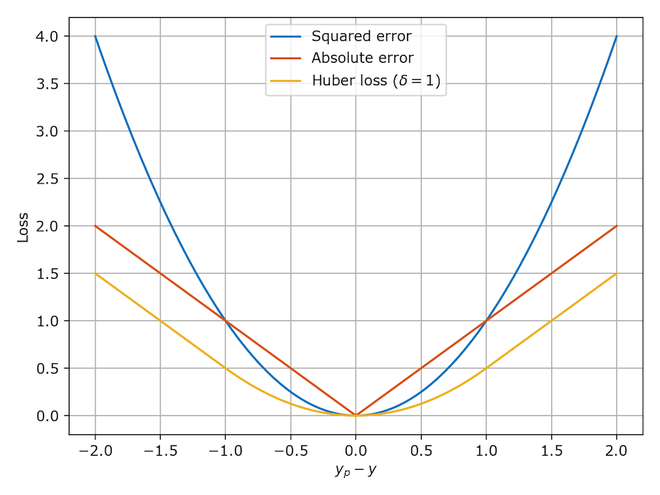
\includegraphics[width=0.7\textwidth]{lossfunctions-660x495.png}
	\caption{مقایسه رفتار توابع خطای مربعات ، خطای مطلق  و زیان هیوبر ($\delta=1$).}
	\label{pic6}
\end{figure}

در این نمودار، محور افقی نشان‌دهنده میزان خطا (تفاضل مقدار پیش‌بینی‌شده و مقدار واقعی) و محور عمودی نشان‌دهنده مقدار زیان است. با بررسی نمودار می‌توان به نتایج زیر دست یافت:

\begin{itemize}
	\item \textbf{خطای مربعات (منحنی آبی):} این تابع رشد سهموی دارد. برای خطاهای بزرگتر از $1$ یا کوچکتر از $-1$، مقدار زیان به شدت افزایش می‌یابد که نشان‌دهنده حساسیت بالای میانگین مربعات خطا به داده‌های پرت است.
	\item \textbf{خطای مطلق (منحنی قرمز):} این تابع به صورت خطی رشد می‌کند. شیب ثابت این تابع باعث می‌شود در برابر داده‌های پرت مقاوم‌تر باشد، اما مشتق‌ناپذیری آن در نقطه صفر می‌تواند در فرآیند بهینه‌سازی چالش‌برانگیز شود.
	\item \textbf{زیان هیوبر (منحنی زرد):} در بازه $[-1, 1]$ رفتار منحنی مشابه تابع مربعات است که بهینه‌سازی را هموار می‌کند، اما در خطاهای بزرگتر، رفتار آن مشابه خطای مطلق می‌شود تا در برابر داده‌های پرت مقاومت کند.
\end{itemize}


\section{معادله نرمال}\label{sec:3-4}
علاوه بر روش‌های تکرارشونده مانند الگوریتم گرادیان کاهشی، برای یافتن پارامترهای بهینه ($\theta$) در مسائل رگرسیون خطی می‌توان از یک راهکار تحلیلی و مستقیم به نام معادله نرمال\LTRfootnote{Normal Equation} استفاده کرد. 

با صفر قرار دادن مشتق تابع هزینه رگرسیون ریج نسبت به بردار $\theta$، به رابطه \eqref{eq13} که در \tablename~\ref{tbl} آورده شده است، دست می‌یابیم. در این رابطه $X$ ماتریس ویژگی‌ها، $y$ بردار مقادیر هدف و $I$ ماتریس همانی است. 
اضافه شدن عبارت $\lambda I$ (مربوط به جریمه ریج) علاوه بر جلوگیری از بیش‌برازش، یک مزیت مهم دیگر نیز دارد: این عبارت تضمین می‌کند که ماتریس $(X^T X + \lambda I)$ همواره معکوس‌پذیر باشد، حتی اگر تعداد ویژگی‌ها از تعداد نمونه‌های آموزشی بیشتر باشد. با این حال، محاسبه معکوس ماتریس از نظر محاسباتی برای داده‌های بسیار بزرگ هزینه‌بر است و در چنین مواقعی استفاده از گرادیان کاهشی ترجیح داده می‌شود.

\section{الگوریتم‌های بهینه‌سازی}\label{sec:3-5}
در کنار انتخاب توابع زیان مناسب، نحوه کمینه‌سازی این توابع نیز از اهمیت بالایی برخوردار است. الگوریتم‌های بهینه‌سازی وظیفه دارند تا با به‌روزرسانی مکرر پارامترهای مدل، مقدار تابع زیان را به حداقل برسانند. انتخاب الگوریتم مناسب می‌تواند تأثیر چشمگیری بر سرعت همگرایی و کیفیت نهایی مدل داشته باشد. 

در \tablename~\ref{tb2} ، مقایسه‌ای بین چند الگوریتم پرکاربرد در یادگیری عمیق و ماشین ارائه شده است. همان‌طور که مشاهده می‌شود، الگوریتم‌های پیشرفته‌تری مانند آدام با وجود نیاز به حافظه کمی بیشتر، سرعت همگرایی بالاتری داشته و در برابر نویز داده‌ها مقاوم‌تر هستند.\cite{kingma2014adam}

\begin{table}[H]
	\centering
	\caption{مقایسه الگوریتم‌های بهینه‌سازی مختلف}
	\label{tb2}
	\renewcommand{\arraystretch}{1.5}
	\setlength{\tabcolsep}{10pt}
	\setlength{\arrayrulewidth}{0.8pt}
	
	\begin{tabular}{|c!{\color{blue}\vrule width 2pt}c|c|c|}
		\hline
		\rowcolor{blue!20}
		نام الگوریتم & سرعت همگرایی & نیاز به حافظه & حساسیت به نویز \\
		\Xhline{3pt}
		
		گرادیان کاهشی استاندارد & کند & کم & زیاد \\
		\hline
		
		\rowcolor{blue!10}
		گرادیان کاهشی تصادفی & متوسط & کم & بسیار زیاد \\
		\hline
		
		الگوریتم آدام & بسیار سریع & متوسط & کم \\
		\hline
	\end{tabular}
\end{table}

\section{معیارهای ارزیابی مدل‌ها}\label{sec:3-6}
پس از آموزش مدل با استفاده از توابع زیان و الگوریتم‌های بهینه‌سازی مناسب، گام بعدی ارزیابی عملکرد مدل بر روی داده‌های آزمون است. معیارهای ارزیابی به ما کمک می‌کنند تا میزان تعمیم‌پذیری مدل را سنجیده و در صورت نیاز، فرایند تنظیم ابرپارامترها را انجام دهیم. بسته به نوع مسئله (رگرسیون یا دسته‌بندی)، از معیارهای متفاوتی استفاده می‌شود.

\subsection{معیارهای ارزیابی در مسائل رگرسیون}\label{subsec:3-6-1}
در مسائل رگرسیون، هدف پیش‌بینی یک مقدار پیوسته است. بنابراین، معیارهای ارزیابی معمولاً بر اساس فاصله بین مقادیر واقعی و مقادیر پیش‌بینی‌شده بنا می‌شوند. دو معیار بسیار پرکاربرد در این زمینه عبارتند از:

\textbf{میانگین مربعات خطا:} این معیار میانگین مربعات اختلاف بین مقادیر واقعی و پیش‌بینی‌شده را محاسبه می‌کند. به دلیل توان دوم، این معیار خطاهای بزرگتر را با شدت بیشتری جریمه می‌کند.
\begin{equation} \label{eq15}
	\mathrm{MSE} = \frac{1}{n} \sum_{i=1}^{n} (y_i - \hat{y}_i)^2
\end{equation}

\textbf{میانگین قدر مطلق خطا:} این معیار میانگین اندازه خطای مطلق را نشان می‌دهد و بر خلاف معیار قبلی، حساسیت کمتری نسبت به داده‌های پرت دارد.
\begin{equation} \label{eq16}
	\mathrm{MAE} = \frac{1}{n} \sum_{i=1}^{n} |y_i - \hat{y}_i|
\end{equation}

\subsection{معیارهای ارزیابی در مسائل دسته‌بندی}\label{subsec:3-6-2}
در مسائل دسته‌بندی، خروجی مدل یک کلاس گسسته یا احتمالی از تعلق به یک کلاس است. در اینجا معیارهای ارزیابی بر اساس تعداد پیش‌بینی‌های درست و نادرست تعریف می‌شوند. 

\textbf{دقت:} ساده‌ترین معیار ارزیابی است که نسبت تعداد پیش‌بینی‌های صحیح به کل داده‌ها را نشان می‌دهد. اگرچه این معیار شهود خوبی ارائه می‌دهد، اما در صورت نامتوازن بودن کلاس‌ها معیار مناسبی نیست.

\textbf{آنتروپی متقاطع:} این معیار که اغلب به عنوان تابع زیان نیز استفاده می‌شود، برای ارزیابی خروجی‌های احتمالی مدل‌های دسته‌بندی (مانند رگرسیون لجستیک یا شبکه‌های عصبی) کاربرد فراوانی دارد. رابطه آن برای یک مسئله چندکلاسه به صورت زیر است:
\begin{equation} \label{eq17}
	\mathrm{CE} = - \sum_{i=1}^{C} y_i \log(\hat{y}_i)
\end{equation}
که در آن $C$ تعداد کلاس‌ها، $y_i$ برچسب واقعی و $\hat{y}_i$ احتمال پیش‌بینی‌شده برای کلاس $i$ است.

همانطور که در روابط \eqref{eq15} تا \eqref{eq17} مشاهده می‌شود، انتخاب معیار ارزیابی وابستگی مستقیمی به ماهیت داده‌ها و هدف نهایی مسئله دارد.




